\chapter{Project Planning}
\label{Chapter3}

\section{Schedule}
\subsection{Estimated project duration}
For this project there have been estimated 450 hours of work, starting on \textbf{19th of February} and ending on \textbf{23th of June}.\\

\subsection{Considerations}
The original plan could be modified to be adapted to deviations. Agile methodology implies that some new requirements can appear which could modify the planning. It is hard to do a realistic planning with Agile methodology because the iteration's requirements are not fully known until the Planning stage.\\

Because this project will be developed sequentially by only one person, the realization of a PERT diagram has been discarded. Nevertheless, some part of the documentation will be done in parallel.

\section{Resources}
For the development of this project, three types of resources will be needed.
\subsection{Human Resources}
\begin{itemize}
	\item One person working 20 hours per week until the finalization of the project.
\end{itemize}
\subsection{Material Resources}
\begin{itemize}
	\item Lenovo IdeaPad U330T\\
	This laptop will be used to write the documentation and develop the project.
\end{itemize}
\subsection{Software Resources}
\begin{itemize}
	\item Trello: Web application to manage project tasks.
	\item teXstudio: LateX editor to write all the documentation.
	\item e-mail: Communication tool used to contact the supervisor. 
	\item Atom: Text editor to write the code.
	\item Git: VCS to backup and keep tracking of the project.
	\item C++: Language used for the development.
	\item PBLib: C++ library for Pseudo-Boolean encodings.
	\item CLion: Code editor focused on C++.
	\item Google Test: Unit testing framework for C++ developed by Google.
\end{itemize}

\section{Project Planning}

\subsubsection{GEP}
This task corresponds to the work done during the GEP course. This task has not any dependency but the work done will be used for the final documentation.\\

The estimated time for this stage is 70 hours.
\subsubsection{Initial Stage}
This stage will be used for defining the requisites to accomplish, the architecture of the software and refactor the previous code. Also, the required tools will be installed. \\

The estimated time for this stage is 90 hours.
\subsubsection{Iterations}
Because Agile methodology will be followed, the project has been divided into iterations. There will be a total of 3 iterations: Pseudo-Boolean minimization, Timeout strategies, and multithreading.\\

For each iteration, 80h of work are estimated.
\paragraph{Planning}\\
This stage will be used for defining the scope of the iteration and goals.\\

This stage will be 10 hours long.
\paragraph{Development and TDD}\\
In this stage, the iteration will be developed and tested.\\

This stage will be 60 hours long.
\paragraph{Finalization}\\
In this stage, all possible bugs will be solved and feedback from the supervisor will be taken.\\

This stage will be 10 hours long.


\subsubsection{Final Stage}
Here, all the development will be finished and it will be used for finishing all the documentation and prepare the final presentation.\\

This stage will take 50 hours.

\subsection{Gantt Diagram}
\begin{figure}[hbtp] 
	\centering
	\makebox[\textwidth]{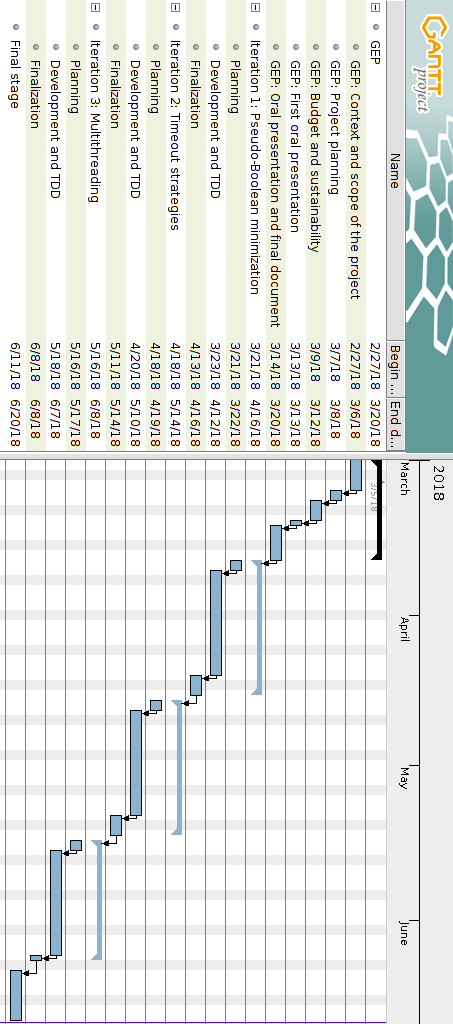
\includegraphics[height=.60\paperheight]{Figures/GanttTable2.png}}
	\caption{Gantt diagram of the project}
	\label{GanttDiagram}
\end{figure}


\section{Alternatives and Action Plans}
Because of using an Agile methodology, the project functionalities can be easily adapted during the development. 

\subsection{Potential deviations}
\subsubsection{Incorrect estimations}
It could be that the estimations are not correct and be under or over estimated. In the first case, the next iteration will be started. On the other case extra hours, for example, weekends, will be used.

